\documentclass[main.tex]{subfiles}
\begin{document}
% neue TOC:
% \begin{itemize}
%     \item DONE wie im konzept gesagt vergleichen wir algorithmen um \$FRAGE zu beantworten
%     \item DONE zunächst definieren wir, wie und woran wir die performanz der algos vergleichen
%     \begin{itemize}
%         \item DONE Wir werden die performanz an 3 metriken messen: P,R,F1 (siehe BG section)
%     \end{itemize}
%     \item wie im konzept festgestellt, sind die pdas nicht vergleichbar. daher haben wir 2 verschiedene datensätze rausgesucht und oder erstellt:
%     \begin{itemize}
%         \item 2D 3D S: statisch, direkt ganze wolke da
%         \item FIN: dynamisch, inkrementell aufbauend
%     \end{itemize}
%     \item wir führen experimente auf beiden datensätzen durch 
%     \item im anschluss werten wir die ergebnisse aus und evaluieren inwiefern die algorithmen echtzeitfähig sind
% \end{itemize}

\chapter{Evaluation}

In diesem kapitel werden zuvor ausgewählte algorithmen einheitlich verglichen und die resultierenden ergebnisse ausgewertet.

\section{Protocol}
% \begin{itemize}
%     \item was wir zeigen wollen
%     \item daher vergleichen wir algorithmen
%     \item wie vergleichen wir, woran ziehen wir schlüsse? 
% \end{itemize}
This work aims to determine which plane detection algorithm is the most suitable for an AR/VR system. For this decision, we uniformly compare the algorithms
selected in Chapter~\ref{chap:Concept}. We split the comparison into two experiments that are conducted on different datasets, namely the 3D-2D-S and the 
self-created FIN dataset. Since the datasets are inherently different, we conduct the experiments and the evaluation thereof separately and 
Wir möchten in dieser arbeit entscheiden können, welcher algorithmus am besten für ein AR/VR system geeignet ist. Dafür machen wir einen einheitlichen
vergleich von den im konzept ausgewählten algorithmen. Wir teilen den Vergleich in zwei experimente auf verschiedenen Datensätzen auf, namely den
3D-2D-S und den selbsterstellten FIN Datensatz. Da beide Datensätze grundsätzlich verschieden aufgebaut sind werden wir sowohl die Experimente, als auch die
Auswertung getrennt vornehmen
und im Anschluss die Ergebnisse in Bezug stellen. Zunächst werden die benutzten Metriken vorgestellt, gefolgt von den Experimenten.


% In this work, we perform a uniform comparison of plane detection algorithms. This comparison aims to evaluate the real-time plane 
% detection on off-the-shelf hardware through the selection of the best algorithm.
% In the following subsection, we present the metrics used for the evaluation.
% We conduct experiments on both datasets and compare the results of both experiments with respect to the real-time applicability of the
% algorithms. Particularly interesting are the differences resulting from the temporal component.
% Finally, by evaluating the results of both experiments, we determine the most suitable plane detection algorithm for real-time, indoor environments. 

\subsection{Metrics}
To quantify the accuracy of the plane detection algorithms, we use the detected planes and the created ground truth to calculate the three following
performance metrics: Precision, Recall, and the F1-score. The procedure of calculation is taken from ~\cite[Section~4]{Araújo_Oliveira_2020} and outlined
in Section~\ref{sec:metrics}.

In addition to the accuracy of an algorithm, we precisely measure the calculation time by splitting the calculation, if possible,
into pre-processing, plane detection, and post-processing (i.e. refinement steps).
(i.e. octree construction, normal calculation)



\subsection{3D-2D-S Experiment}
Wir schmeissen alle algorithmen auf alle segmentierten scenen des 3D-2D-S Datensatzes. Bei manchen algorithmen haben wir bestimmte parameter
angepasst um die ergebnisse zu verbessern.

\paragraph{OPS}
Durch empirisches Testen ergab sich eine kombination der folgenden Parameterwerte.
\begin{table}[H]
    \centering
    \resizebox{0.7\textwidth}{!}{%
        \begin{tabular}{c|ccccc}
            Parameter & $\alpha_s$ & $KNN$ & $\theta_{h}$ & $\theta_{N}$ & $p$  \\ \hline
            Value     & 0.03       & 30    & 0.05         & 100          & 0.99
        \end{tabular}%
    }
    \caption{}
    \label{tab:3d2ds-ops}
\end{table}

\paragraph{3D-KHT}
Durch empirisches Testen ergab sich eine kombination der folgenden Parameterwerte.
% FIXME im background sicher gehen dass ich die erklärt habe
\begin{table}[H]
    \centering
    \resizebox{0.7\textwidth}{!}{%
        \begin{tabular}{c|ccccccc}
            Parameter & $\phi_{num}$ & $\rho_{num}$ & $s_{level}$ & $s_{ps}$ & $d_{max}$ & $s_\alpha$ & $s_\beta$ \\ \hline
            Value     & 30           & 200          & 2           & 0.002    & 0.08      & 18         & 6
        \end{tabular}%
    }
    \caption{}
    \label{tab:3d2ds-3dkht}
\end{table}


\subsection{FIN Experiment}
Auch im dynamischen experiment auf dem FIN datensatz lassen wir alle algorithmen jeden zeitschritt berechnen.
Hierbei ist es wichtig, bestimmte parameter der Algorithmen den höheren leveln von noise anzupassen.

\paragraph{OPS}
Durch empirisches Testen ergab sich eine kombination der folgenden Parameterwerte.
\begin{table}[H]
    \centering
    \resizebox{0.7\textwidth}{!}{%
        \begin{tabular}{c|ccccc}
            Parameter & $\alpha_s$ & $KNN$ & $\theta_{h}$ & $\theta_{N}$ & $p$  \\ \hline
            Value     & 0.03       & 90    & 0.35         & 100          & 0.99
        \end{tabular}%
    }
    \caption{}
    \label{tab:fin-ops}
\end{table}

\paragraph{3D-KHT}
Durch empirisches Testen ergab sich eine kombination der folgenden Parameterwerte. Bemerkenswert sind die veränderungen der parameter $\rho_{num}$ und
$s_\alpha$. Die intuition hinter dem letzteren Wert ist, dass je kleiner $s_\alpha$ ist, desto dicker sind die erwarteten ebenen im datensatz, i.e., desto
mehr noise ist vorhanden. Es war ebenso nötig die $\rho$ Diskretisierung $\rho_{num}$ zu reduzieren, da sonst zu viele falsche ebenen gefunden werden würden.

% FIXME im background sicher gehen dass ich die erklärt habe
\begin{table}[H]
    \centering
    \resizebox{0.7\textwidth}{!}{%
        \begin{tabular}{c|ccccccc}
            Parameter & $\phi_{num}$ & $\rho_{num}$ & $s_{level}$ & $s_{ps}$ & $d_{max}$ & $s_\alpha$ & $s_\beta$ \\ \hline
            Value     & 30           & 100          & 2           & 0.002    & 0.1       & 8          & 6
        \end{tabular}%
    }
    \caption{}
    \label{tab:fin-3dkht}
\end{table}

\section{Results}
This section deals with the results of the experiments. The individual results of both experiments are presented and analyzed.

\subsection{Results 2D-3D-S Experiments}
% FIXME redo this table
\begin{table}[H]
    \centering
    \begin{tabular}{c|cccc}
              & Precision & Recall & F1   & Time(s) \\ \hline
        RSPD  & 0.85      & 0.89   & 0.86 & 0.90    \\
        OPS   & 0.87      & 0.70   & 0.77 & 16.75   \\
        3DKHT & 0.75      & 0.43   & 0.53 & 0.91    \\
        OBRG  & 0.77      & 0.69   & 0.72 & 44.66
    \end{tabular}
    \caption[Overall 2D-3D-S Results]{Average results of each algorithm over the 2D-3D-S dataset.}
    \label{tab:algo-acc}
\end{table}

Every algorithm performs calculations on every scene included in 2D-3D-S.
The results of each algorithm on an individual scene type are reported in Figure~\ref{fig:stanfordaccuracy} and Figure~\ref{fig:violintime}. As shown in Table~\ref{tab:algo-acc},
RSPD produces the overall best results with an average of 85\% precision, 89\% recall and an F1-score of 86\%, as well as an average of 0.9 seconds of calculation time.
The only other algorithm that achieves similar calculation times is 3D-KHT, which takes 0.91 seconds on average. Considering our definition of \textit{real-time} in Section~\ref{sec:realtime},
RSPD and 3D-KHT are able to perform plane detecion in real-time. Still, 3D-KHT produces the worst overall accuracy results with an average precision of 75\%, recall of 43\%, and an F1-score of 53\%.

With an average of about 17 seconds(OPS) and about 44 seconds(OBRG), both algorithms do not achieve real-time plane detection (see Table~\ref{tab:algo-acc}).


\begin{figure}[]
    \centering
    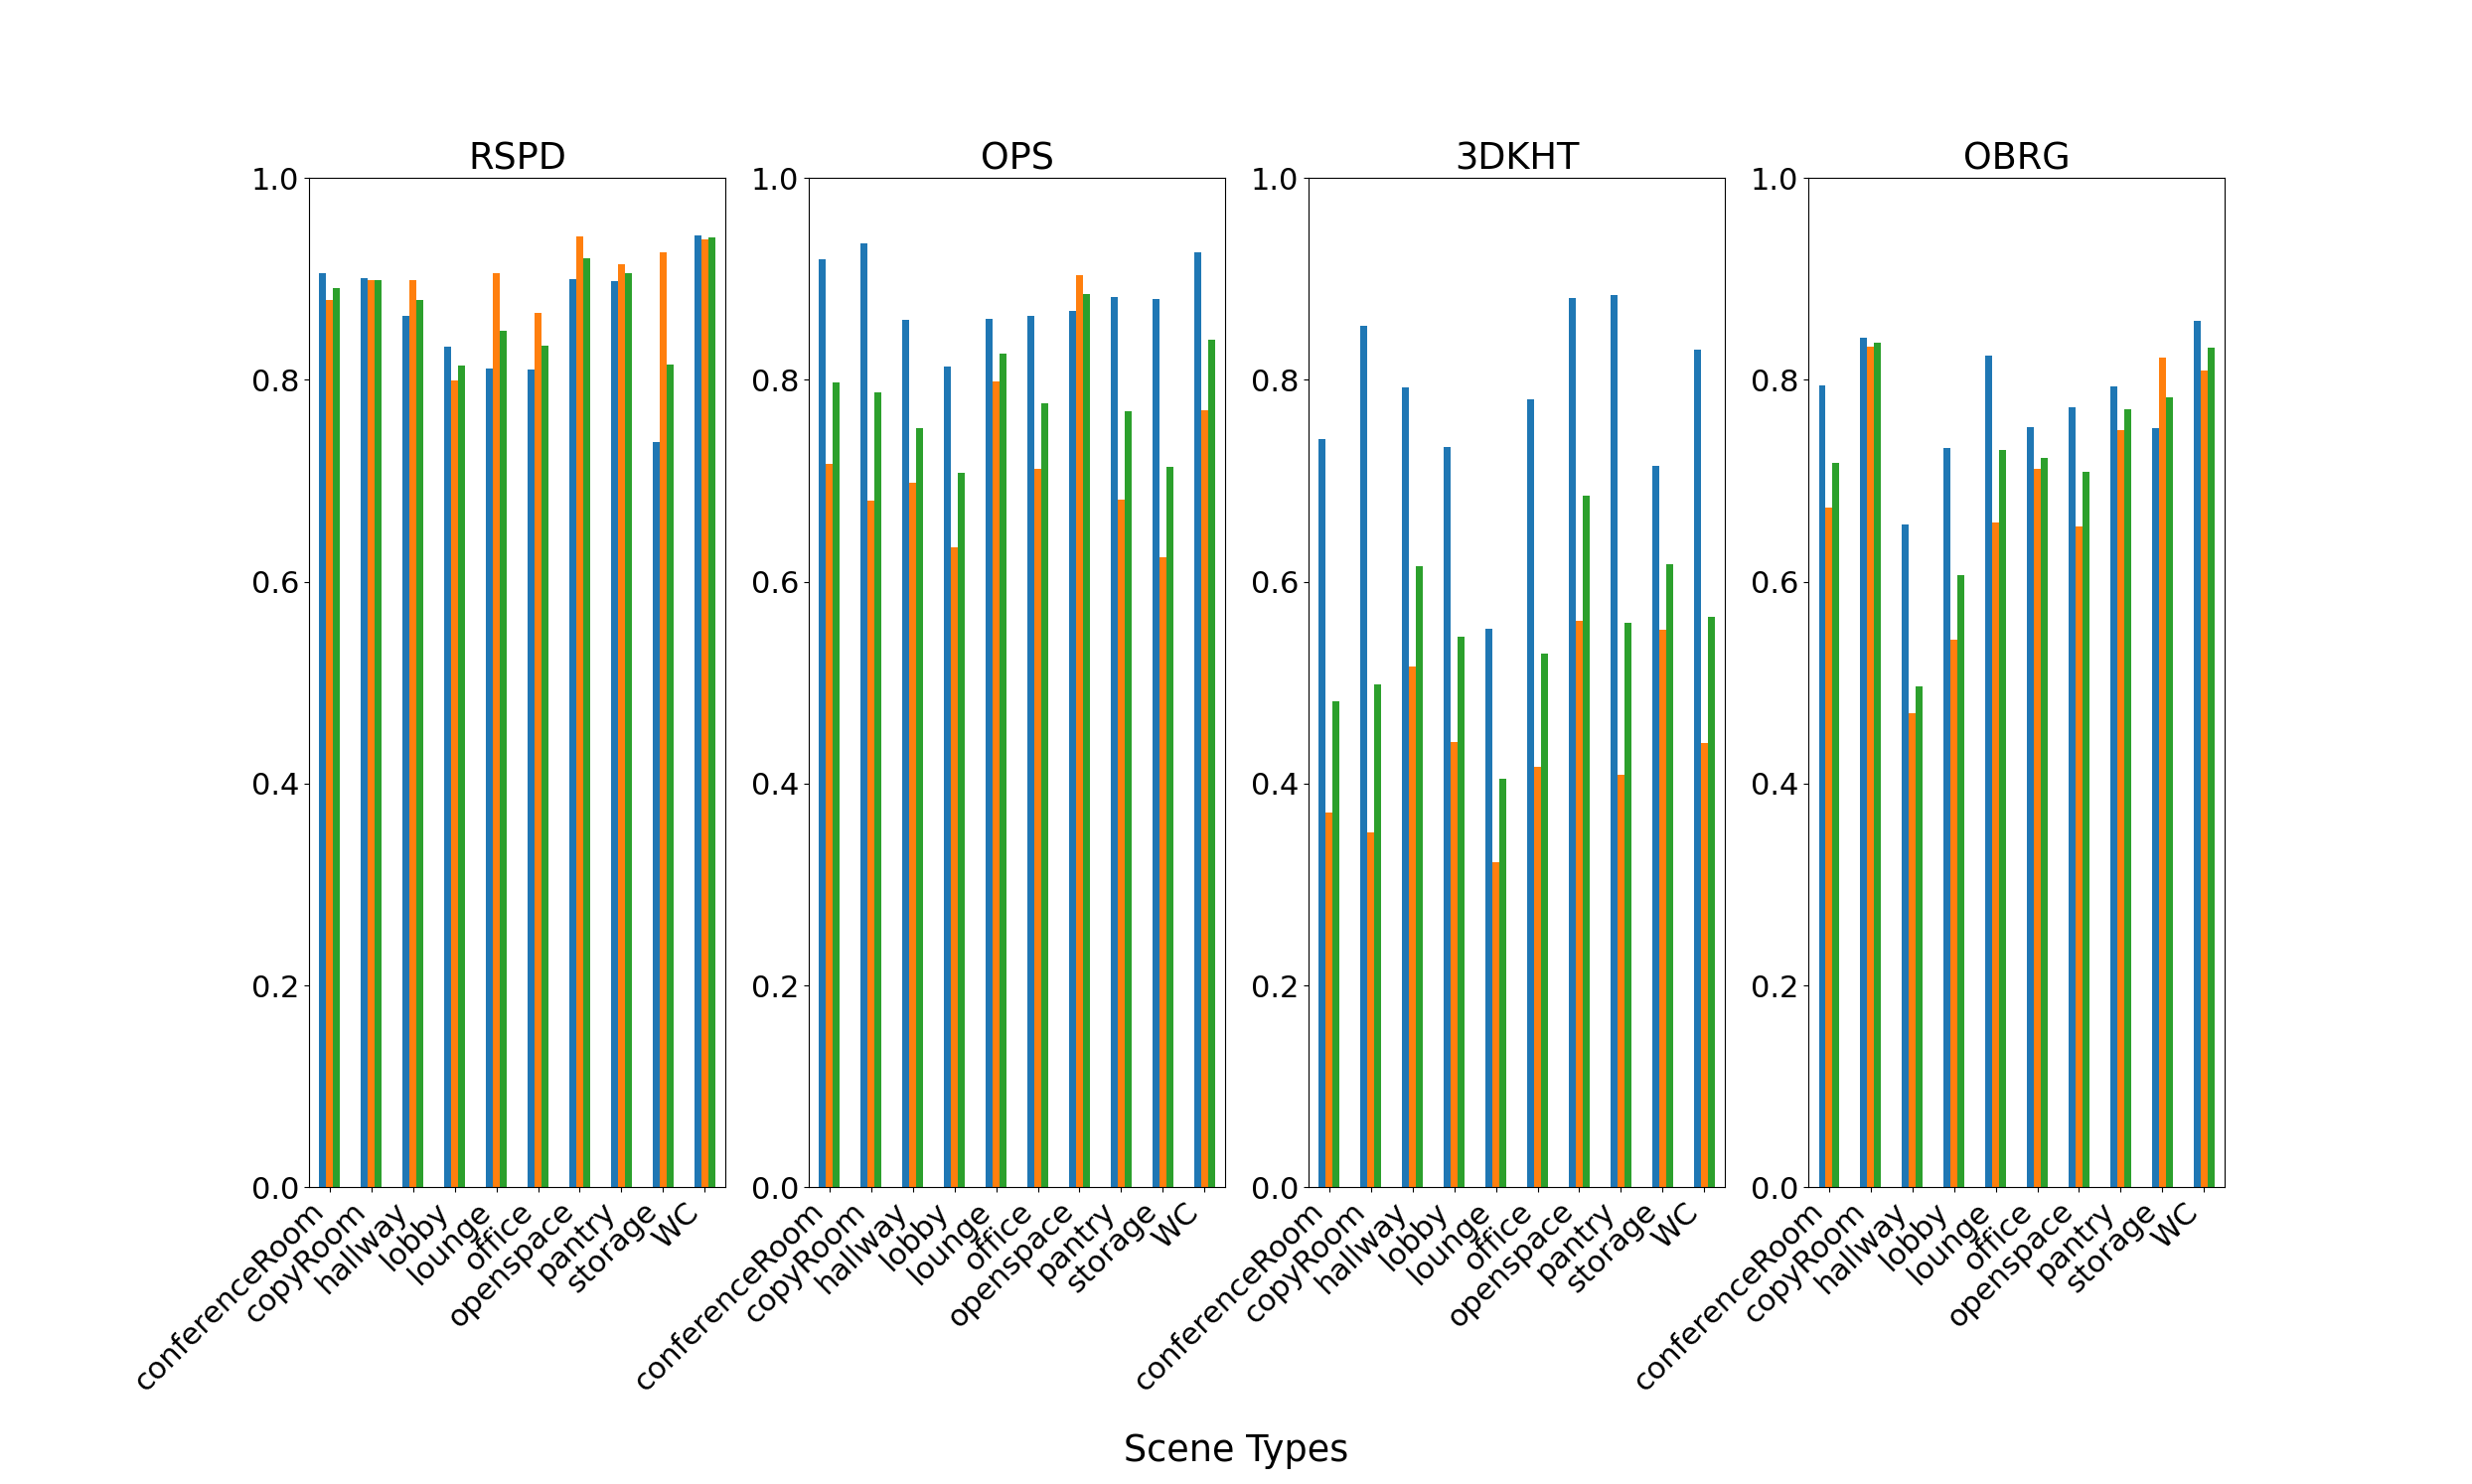
\includegraphics[width=15 cm]{images/accuracy_total.png}
    \caption[Accuracy Results 2D-3D-S]{Average Accuracy for each scene type. The Precision
        is colored blue, recall is orange and the F1-score is green.}
    \label{fig:stanfordaccuracy}
\end{figure}

\begin{figure}[]
    \centering
    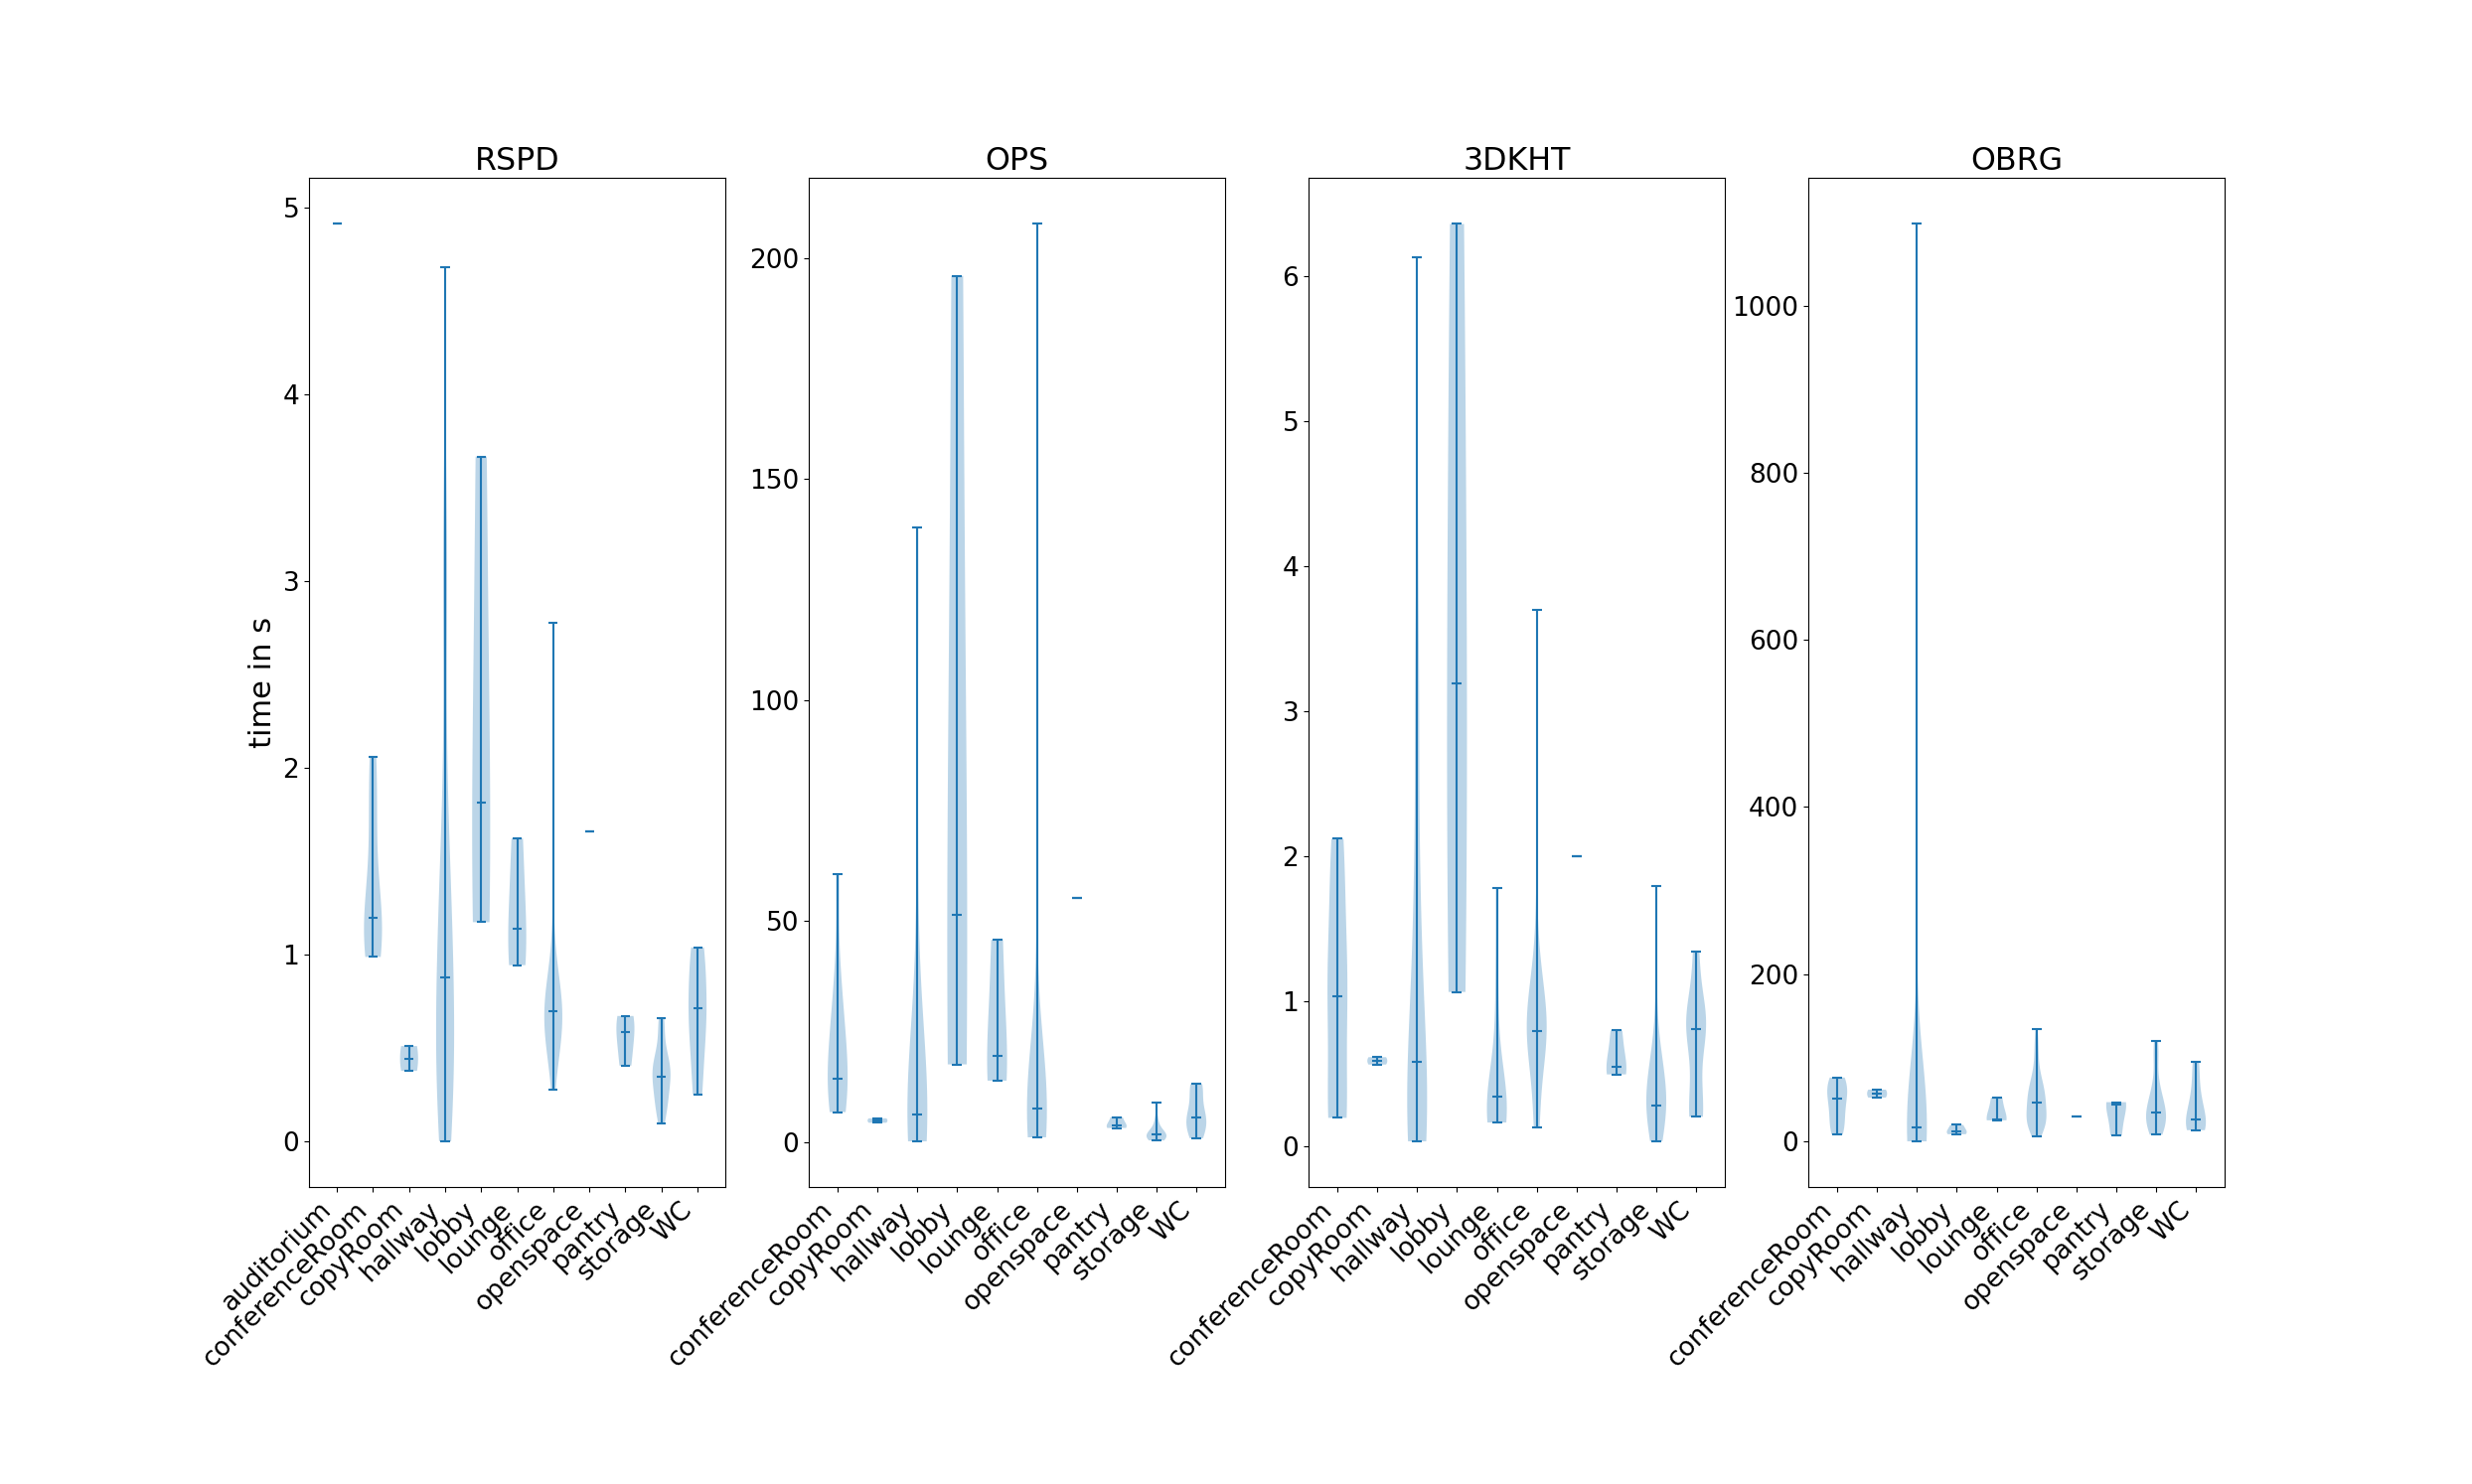
\includegraphics[width=15 cm]{images/times_violin.png}
    \caption[Time Results 2D-3D-S]{Times per scene type. The lowest tick denotes the minimum time, the highest
        denotes the maximum time spent in the calculation. The middle tick shows the mean time.
        Note, that the plots
        do not share the same y-axis.}
    \label{fig:violintime}
\end{figure}

\subsection{Results Real-Life Experiments}
\textit{So far:}

\begin{figure}[]
    \centering
    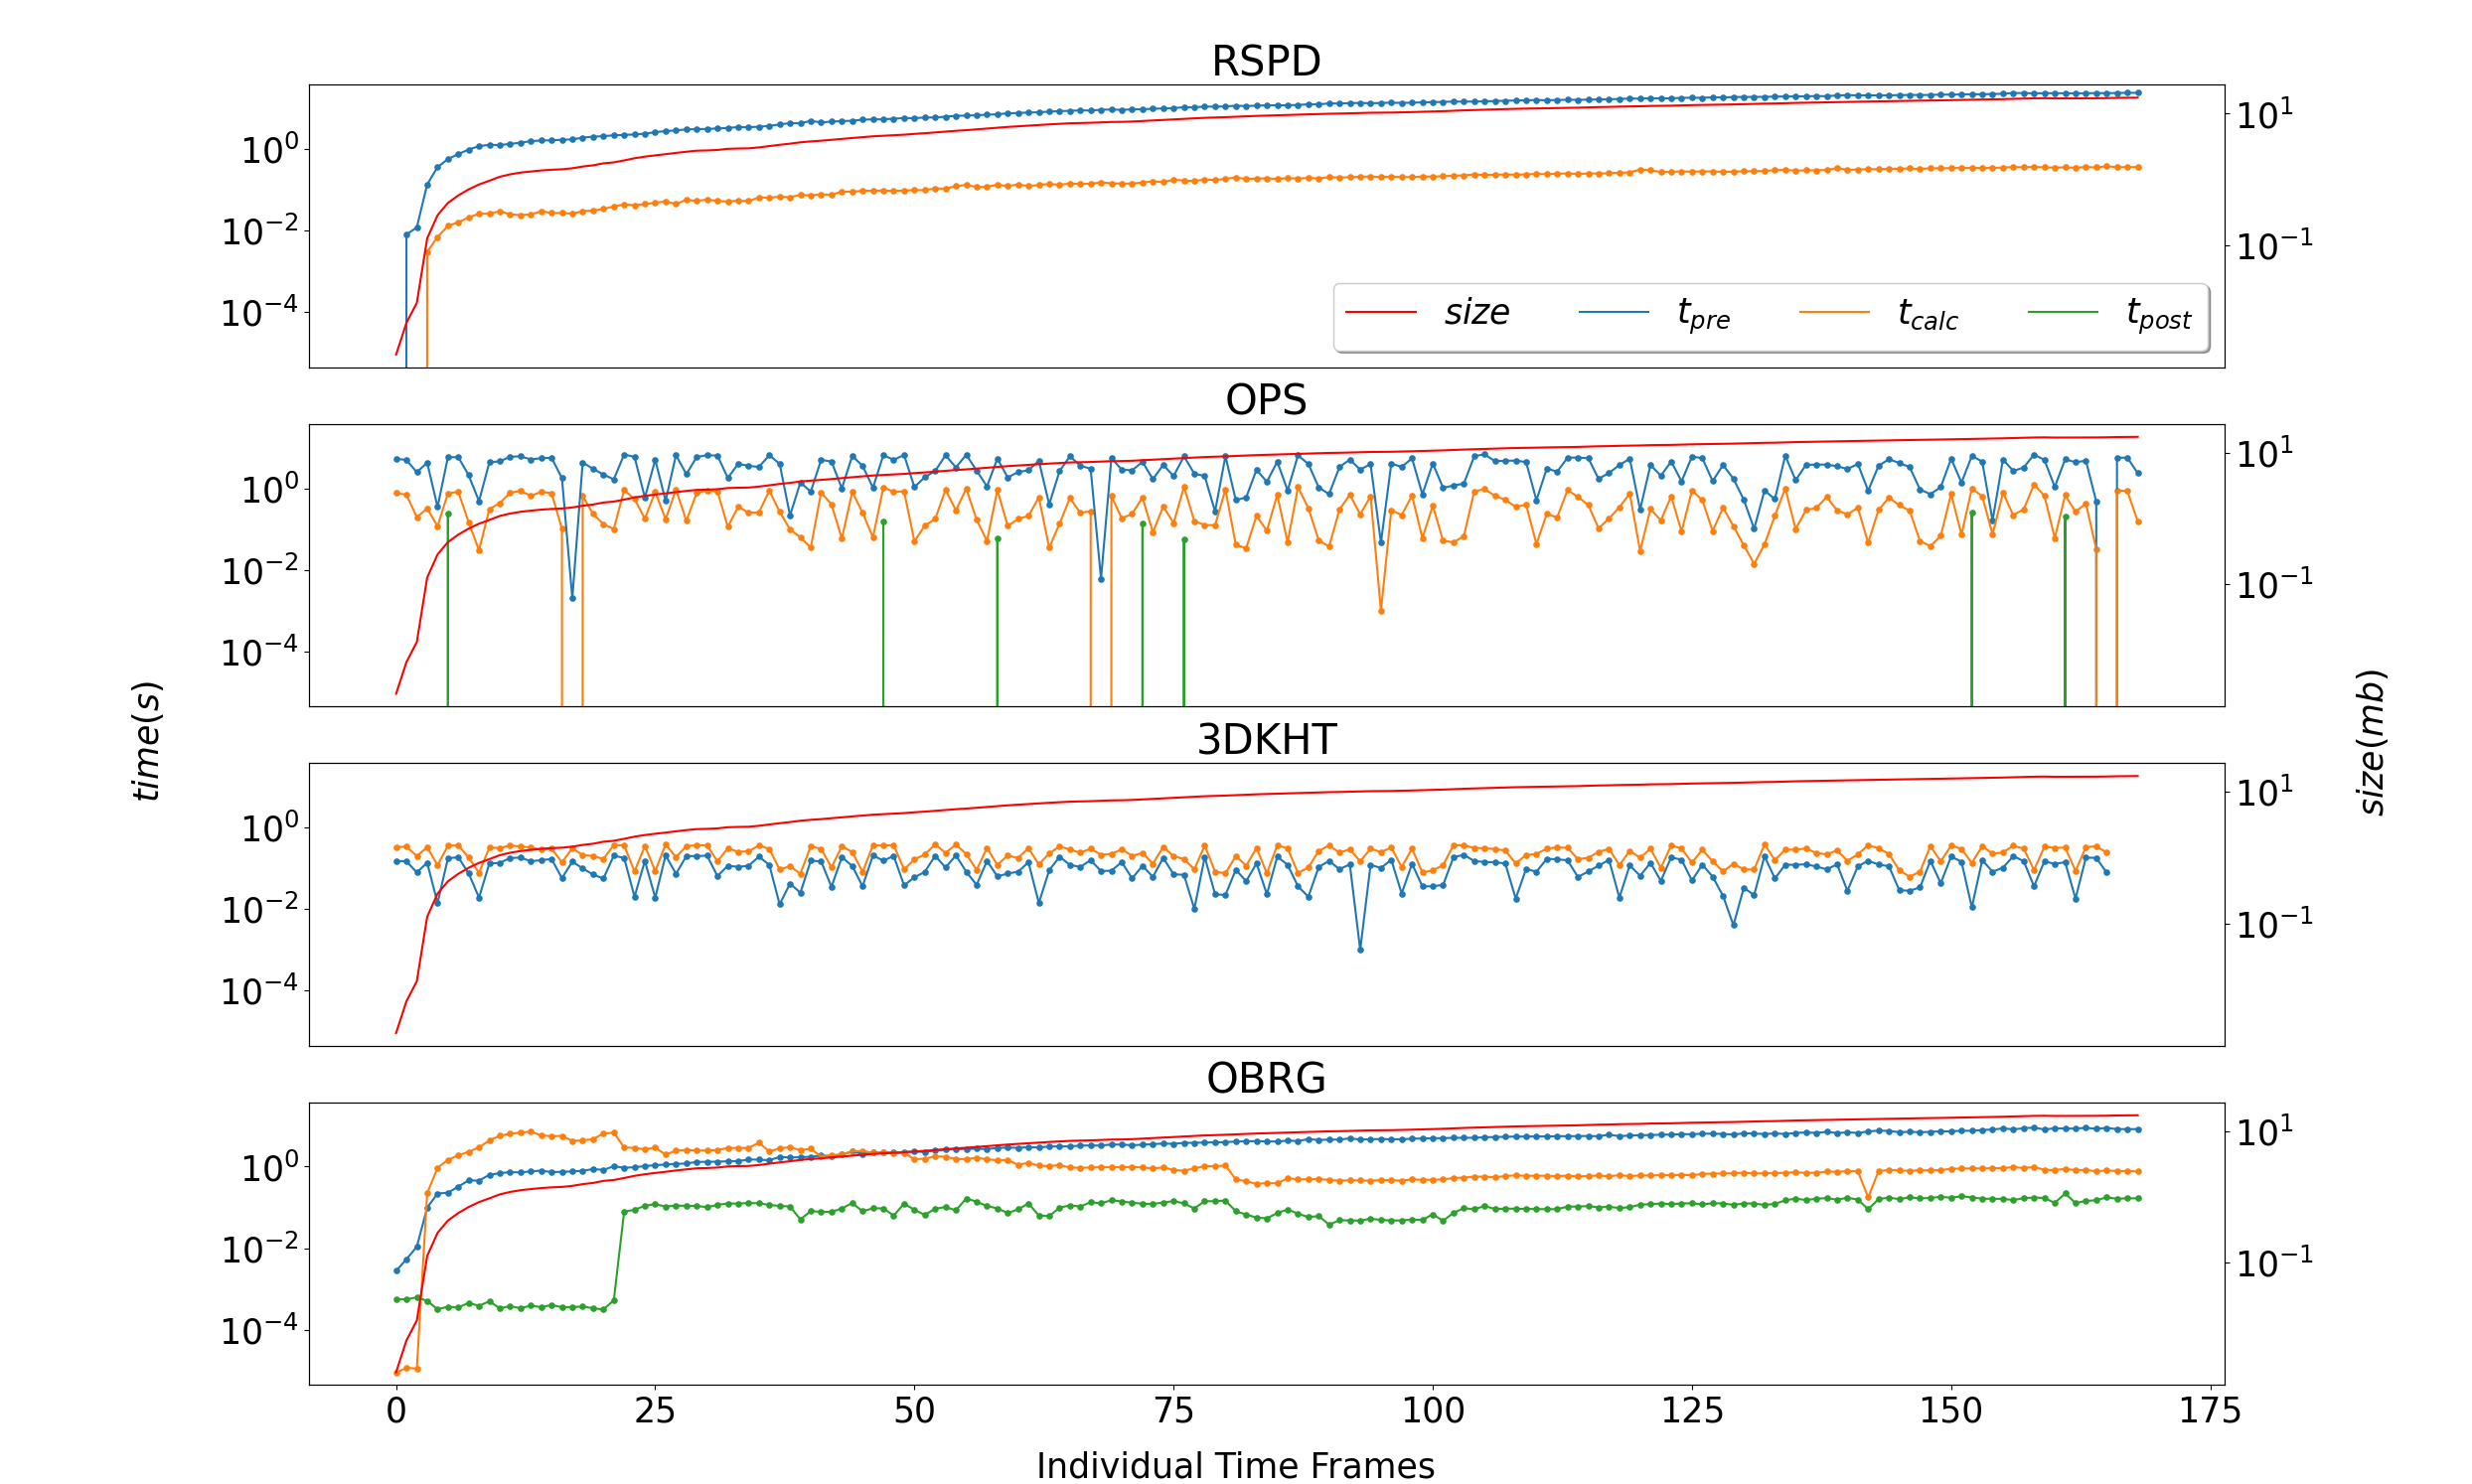
\includegraphics[width=\textwidth]{images/dyn_time-hallway.png}
    \caption[Time Results Hallway]{Calculation times(blue) of the hallway scene and cloud size(red) of each time step.}
    \label{fig:dynhallway}
\end{figure}

The calculation times of all algorithms except OBRG seem to be proportional to the size of the point cloud.
% TODO similar figure for 2D-3D-S
The quality of plane detection, however, decreases dramatically in comparison to the Stanford Datasets. RSPD is the only dataset that
is able to detect planes. %(see Figure~\ref{fig:}). 


\begin{table}[]
    \centering
    \begin{tabular}{c|ccc}
               & Precision          & Recall             & F1-Score           \\ \hline
        RSPD   & 0.39               & 0.50               & 0.44               \\
        OPS    & 0.47               & 0.31               & 0.37               \\
        3D-KHT & 0.32               & 0.32               & 0.32               \\
        OBRG   & \textcolor{red}{0} & \textcolor{red}{0} & \textcolor{red}{0}
    \end{tabular}%
    \caption{Average Results for the auditorium scene of the FIN dataset.}
    \label{tab:res-fin-audi}
\end{table}

\begin{table}[]
    \centering
    \begin{tabular}{c|ccc}
               & Precision          & Recall             & F1-Score           \\ \hline
        RSPD   & 0.58               & 0.63               & 0.60               \\
        OPS    & 0.69               & 0.29               & 0.40               \\
        3D-KHT & 0.47               & 0.46               & 0.46               \\
        OBRG   & \textcolor{red}{0} & \textcolor{red}{0} & \textcolor{red}{0}
    \end{tabular}%
    \caption{Average Results for the conferenceRoom scene of the FIN dataset.}
    \label{tab:res-fin-conf}
\end{table}

\begin{table}[]
    \centering
    \begin{tabular}{c|ccc}
               & Precision          & Recall             & F1-Score           \\ \hline
        RSPD   & 0.50               & 0.51               & 0.51               \\
        OPS    & 0.87               & 0.20               & 0.32               \\
        3D-KHT & 0.57               & 0.44               & 0.49               \\
        OBRG   & \textcolor{red}{0} & \textcolor{red}{0} & \textcolor{red}{0}
    \end{tabular}%
    \caption{Average Results for the hallway scene of the FIN dataset.}
    \label{tab:res-fin-hall}
\end{table}

\begin{table}[]
    \centering
    \begin{tabular}{c|ccc}
               & Precision                             & Recall                                & F1-Score                              \\ \hline
        RSPD   & 0.60                                  & 0.62                                  & 0.61                                  \\
        OPS    & 0.75                                  & 0.37                                  & 0.49                                  \\
        3D-KHT & 0.62                                  & 0.55                                  & 0.58                                  \\
        OBRG   & \textbackslash{}textcolor\{red\}\{0\} & \textbackslash{}textcolor\{red\}\{0\} & \textbackslash{}textcolor\{red\}\{0\}
    \end{tabular}
    \caption{Average Results for the office scene of the FIN dataset.}
    \label{tab:res-fin-off}
\end{table}

\subsection{Summary Results}
% NOTE 3DKHT kann keine löcher oder non-rectangular ebenen basteln!
This section combines the preceding results of both experiments.
RSPD is the only algorithm that produces comparable results to the Stanford experiment in the dynamic experiment.
The remaining algorithms cannot reliably detect planes in an incrementally growing environment inheriting varying degrees of noise.

The reason for RSPD's dominance is likely caused by the inherent robustness against noise, as described in Section~

Die ergebnisse der beiden experimente unterscheiden sich in folgendem punkt. Dazu sei gesagt, dass die experimente folgende übereinstimmungen haben.
Das lässt sich so erklären. Alternative gründe davon könnten diese hier sein.

Ich denke RSPD ragt heraus, da hier besonders auf noise resistenz geachtet wurde. % TODO verweis auf diverse noise tests im BG


\end{document}